\chapter{Cinématique}
	\section{Vecteur position d'un point d'un solide}
	\begin{definition}
	Soient $t$ la variable de temps et $S$ un solide en mouvement par rapport à un repère $\Rc(O,\vect{x},\vect{y},\vect{z})$. Le vecteur position du point $P(t)$ du solide dans le repère \Rc{} à la date $t$ est le vecteur $\vect{OP}(t)$ avec $O$ origine de \Rc{}.
	\end{definition}
	
	\section{Vecteur vitesse d'un point d'un solide}
	\begin{definition}
		Le vecteur vitesse d'un point $P(t)$ du solide $S$ par rapport au repère \Rc{}, à la date $t$, est la dérivée par rapport à $t$ du vecteur position $\vect{OP}(t)$, pour un observateur lié au repère $\Rc$ . On le notera :
		\begin{equation}
			\V[\Rc]{P}{S}=\diff[\Rc{}]{\vect{OP}}
		\end{equation}
	\end{definition}
	
	\section{Vecteur accélération}
	\begin{definition}
	Le vecteur accélération d'un point $P(t)$ du solide $S$ par rapport au repère \Rc{}, à la date $t$, est la dérivée par rapport à $t$ du vecteur vitesse $\vect{OP}(t)$, pour un observateur lié au repère \Rc{}. On le notera :
	\begin{equation}
		\G[\Rc]{P}{S}=\diff[\Rc]{\V[\Rc]{P}{S}}=\left.\frac{\mathrm{d}^2\vect{OP}}{\mathrm{d}t^2}\right|_{\Rc}
	\end{equation}
	\end{definition}
\begin{minipage}[b]{0.5\textwidth}
	Soit $(\mathcal{C})$ la trajectoire de $P(t)$, c'est-à-dire l'ensemble des positions balayées par $P(t)$ au cours du temps. $\V[\Rc]{P}{S}$ et $\G[\Rc]{P}{S}$ présentent alors les propriétés suivantes :
	\begin{itemize}
		\item $\V[\Rc]{P}{S}$ est tangent à $(\mathcal{C})$,
		\item $\G[\Rc]{P}{S}$ est orienté vers l'intérieur de la courbure de $(\mathcal{C})$.
	\end{itemize}
\end{minipage}	
	\begin{minipage}[b]{0.4\textwidth}
		\centering
		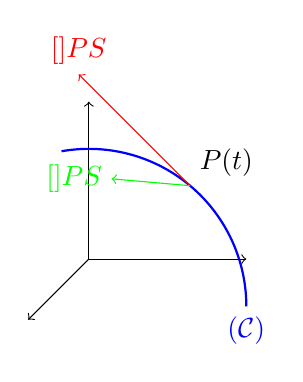
\begin{tikzpicture}[scale=2]
			\node[anchor=east] at (0,0,0) {$\Rc$};
			\draw[<->] (1,0,0) -- (0,0,0) -- (0,1,0);
			\draw[->] (0,0,0) -- (0,0,1);
			\draw[blue,thick] (1,-0.3) arc (-0:100:1) node[pos=0,anchor=north]{$(\mathcal{C})$} coordinate[pos=0.5] (P);
			\draw[->,red] (P) -- ++(135:1) node[anchor=south] {$\V[\Rc]{P}{S}$};
			\draw[->,green] (P) -- ++(175:0.5) node[anchor=east] {$\G[\Rc]{P}{S}$};
			\node[anchor=south west] at (P){$P(t)$};
		\end{tikzpicture}		
	\end{minipage}


	\section{Vecteur vitesse de rotation}
		On suppose deux repères $\Rc(O,\vect{x},\vect{y},\vect{z})$ et $\Rc_1(O_1,\vect{x}_1,\vect{y}_1,\vect{z}_1)$ en mouvement l'un par rapport à l'autre. 
		
		On peut passer de la base $\mathcal{B}(\vect{x},\vect{y},\vect{z})$ à la base $\mathcal{B}_1(\vect{x}_1,\vect{y}_1,\vect{z}_1)$ par une unique rotation. Soient $\vect{u}$ l'axe de cette rotation et $\alpha$ son angle :
		\begin{equation}
			\Rc(\vect{x},\vect{y},\vect{z})\xrightarrow[\alpha]{\vect{u}}(\vect{x}_1,\vect{y}_1,\vect{z}_1)
		\end{equation}
		
		On appelle alors vecteur vitesse de rotation du repère $\Rc_1$ par rapport au repère $\Rc$ le vecteur suivant :
		\begin{equation}
			\Om{\Rc_1}=\dot{\alpha}\vect{u} \quad \text{avec : } \dot{\alpha}=\frac{\mathrm{d}\alpha}{\mathrm{d}t}
		\end{equation}
		
		\begin{note}
De la même façon, on note habituellement $\ddot{\alpha}$ la dérivée seconde de $\alpha$ par rapport au temps :
			\begin{equation}
				\ddot{\alpha}=\frac{\mathrm{d}^2\alpha}{\mathrm{d}t^2}
			\end{equation}
		\end{note}
	
	\section{Calcul des vecteurs vitesse et accélération}
	\begin{theorem}
		\hidden{
		\label{th:derivation}
		Soient $\vect{U}(t)$ un vecteur quelconque et $\Rc(O,\vect{x},\vect{y},\vect{z})$ et $\Rc_1(O,\vect{x}_1,\vect{y}_1,\vect{z}_1)$ deux repères orthonormés directs, $\Rc_1$ étant en mouvement par rapport à \Rc{}. On a alors :	
		\begin{equation}
			\diff[\Rc]{\vect{U}(t)}=\diff[\Rc_1]{\vect{U}(t)}+\Om[\Rc]{\Rc_1}\wedge\vect{U}(t)		
		\end{equation}
		où $\Om[\Rc]{\Rc_1}$ est le vecteur vitesse de rotation.
		}
	\end{theorem}
	
	\begin{proof}
	
		On se place dans le cas où $\vect{z}=\vect{z}_1$. On décompose $\vect{U}(t)$ dans la base $\Rc_1$ :
		\begin{equation}
			\label{eq:decomposition}
			\vect{U}(t)=a(t)\vect{x}_1+b(t)\vect{y}_1+c(t)\vect{z}_1
		\end{equation}	
Soit $\alpha$ l'angle $(\vect{x},\vect{x}_1)=(\vect{y},\vect{y}_1)$.
			
\begin{minipage}[b]{0.3\textwidth}
	\centering
	\tdplotsetmaincoords{70}{110}
	\begin{tikzpicture}[tdplot_main_coords,scale=2.5]
	\draw[thick,->] (0,0,0) -- (1,0,0) node[anchor=north east]{$\vect{x}$};
	\draw[thick,->] (0,0,0) -- (0,1,0) node[anchor=north west]{$\vect{y}$};
	\draw[thick,->] (0,0,0) -- (0,0,1) node[anchor=south]{$\vect{z}$};
	\tdplotsetrotatedcoords{0}{0}{30}
	\draw[thick,color=blue,tdplot_rotated_coords,->] (0,0,0) --	(1,0,0) node[anchor=north]{$\vect{x}_1$};
	\draw[thick,color=blue,tdplot_rotated_coords,->] (0,0,0) --	(0,1,0) node[anchor=west]{$\vect{y}_1$};
	\draw[thick,color=blue,tdplot_rotated_coords,->] (0,0,0) --	(0,0,.7) node[anchor=east]{$\vect{z}_1$};
	\tdplotdrawarc[-stealth]{(0,0,0)}{0.5}{0}{30}{anchor=north}{$\alpha$}
	\tdplotdrawarc[-stealth]{(0,0,0)}{0.5}{90}{120}{anchor=west}{$\alpha$}
	\end{tikzpicture}	
\end{minipage}		
\begin{minipage}[b]{0.65\textwidth}	
		\begin{subequations}
			\label{eq:projection}
			\begin{align}
				\vect{x}_1&=\cos\alpha\vect{x}+\sin\alpha\vect{y}\\
				\vect{y}_1&=-\sin\alpha\vect{x}+\cos\alpha\vect{y}
			\end{align}			
		\end{subequations}
Ainsi :
		\begin{subequations}
			\begin{align}
				\diff[\Rc]{\vect{x}_1}&=\left[\frac{\mathrm{d}\vect{x}_1}{\mathrm{d}\alpha}\frac{\mathrm{d}\alpha}{\mathrm{d}t}\right]_{\Rc}=
					-\dot{\alpha}\sin\alpha\vect{x}+\dot{\alpha}\cos\alpha\vect{y}\\
				\diff[\Rc]{\vect{y}_1}&=\left[\frac{\mathrm{d}\vect{y}_1}{\mathrm{d}\alpha}\frac{\mathrm{d}\alpha}{\mathrm{d}t}\right]_{\Rc}=
					-\dot{\alpha}\cos\alpha\vect{x}-\dot{\alpha}\sin\alpha\vect{y}\\
				\diff[\Rc]{\vect{z}_1}&=0
			\end{align}
		\end{subequations}		
\end{minipage}

		On peut donc écrire :
		\begin{subequations}
			\label{eq:prodvect}
			\begin{align}
				\diff[\Rc]{\vect{x}_1}&=\dot{\alpha}\vect{z}\wedge\vect{x}_1\\
				\diff[\Rc]{\vect{y}_1}&=\dot{\alpha}\vect{z}\wedge\vect{y}_1\\
				\diff[\Rc]{\vect{z}_1}&=\dot{\alpha}\vect{z}\wedge\vect{z}_1
			\end{align}
		\end{subequations}
		
En dérivant terme à terme les composantes de l'équation~\eqref{eq:decomposition}, on trouve :
		\begin{equation}
			\diff[\Rc]{\vect{U}(t)}=a(t)\diff[\Rc]{\vect{x}_1}+b(t)\diff[\Rc]{\vect{y}_1}+c(t)\diff[\Rc]{\vect{z}_1}+
			\dot{a}(t)\vect{x}_1+\dot{b}(t)\vect{y}_1+\dot{c}(t)\vect{z}_1
			\label{eq:produit-vect}
		\end{equation}		
		Soit $\Om[\Rc]{\Rc_1}=\dot{\alpha}\vect{z}$.
		L'équation~\eqref{eq:produit-vect} peut s'écrire sous la forme vectorielle suivante :
		\begin{equation*}
			\diff[\Rc]{\vect{U}(t)}=\Om[\Rc]{\Rc_1}\wedge\Big(a(t)\vect{x}_1+b(t)\vect{y}_1+c(t)\vect{z}_1\Big)+\diff[\Rc_1]{\vect{U}(t)}
		\end{equation*}
	\end{proof}
	
\section{Angles d'Euler}
	\subsection{Définition}
	\label{sec:euler}
\emph{Objectif : décrire de façon unique l'orientation d'une base $\mathcal{B}_1(\vect{x}_1,\vect{y}_1,\vect{z}_1)$ par rapport à un autre base $\mathcal{B}(\vect{x},\vect{y},\vect{z})$.}

On peut passer d'une base à l'autre par trois rotations successives. La convention d'Euler, illustrée en figure~\ref{fig:euler}, nous donne la séquence suivante :
\begin{enumerate}
	\item Précession : $\mathcal{B}(\vect{x},\vect{y},\vect{z})\xrightarrow[\psi]{\vect{z}}(\vect{u},\vect{v},\vect{z})$
	\item Nutation : $(\vect{u},\vect{v},\vect{z})\xrightarrow[\theta]{\vect{v}}(\vect{w},\vect{v},\vect{z}_1)$
	\item Rotation propre : $(\vect{w},\vect{v},\vect{z}_1)\xrightarrow[\varphi]{\vect{z}_1}\mathcal{B}_1(\vect{x}_1,\vect{y}_1,\vect{z}_1)$
\end{enumerate}

\begin{figure}[htbp]
	\centering
		\tdplotsetmaincoords{70}{130}
	\begin{tikzpicture}[tdplot_main_coords,scale=5]
		%% Définition des différents styles
		\tikzstyle{init} = [black]			% base initiale
		\tikzstyle{prec} = [blue]			% 1ere base intermédiaire
		\tikzstyle{nuta} = [red]			% 2eme base initiale
		\tikzstyle{rotp} = [green]			% base finale
		\tikzstyle{base} = [thick,-stealth]	% Tracé des bases
		\tikzstyle{angle} = [thick,-latex]	% Tracé des arcs pour les angles
		\tikzstyle{circle} = [thin,dashed]	% Tracé des cercles
		
		%% Paramètres géométriques		
		\def\epsi{15}	% Angle de precession dessiné
		\def\etheta{15}	% Angle de nutation dessiné
		\def\ephi{15}	% Angle de rotation propre dessiné
		\def\rang{0.7}	% Rayon utilisé pour tracer les angles
		
		%% Tracé
		% Repère initial
		\coordinate (O) at (0,0,0);
		\draw[base,init] (O) -- (1,0,0) node[anchor=north east]{$\overrightarrow{x}$};
		\draw[base,init] (O) -- (0,1,0) node[anchor=north west]{$\overrightarrow{y}$};
		\draw[base,init] (O) -- (0,0,1) node[anchor=south]{$\overrightarrow{z}$};
		
		% Précession
		\tdplotsetrotatedcoords{\epsi}{0}{0}
		\draw[tdplot_rotated_coords,angle,prec] (O) --(1,0,0) node[anchor=north east]{$\overrightarrow{u}$};
		\draw[tdplot_rotated_coords,angle,prec] (O) --(0,1,0) node[anchor=west]{$\overrightarrow{v}$};
		\tdplotdrawarc[tdplot_rotated_coords,circle,prec]{(0,0,0)}{1}{0}{360}{}{}	
		\tdplotdrawarc[tdplot_rotated_coords,angle,prec]{(0,0,0)}{\rang}{90-\epsi}{90}{anchor=north east,prec}{$\psi$}	
		\tdplotdrawarc[tdplot_rotated_coords,angle,prec]{(0,0,0)}{\rang}{-\epsi}{0}{anchor=north east,prec}{$\psi$}	

		% Nutation
		\tdplotsetrotatedcoords{\epsi}{\etheta}{0}
		\draw[tdplot_rotated_coords,base,nuta] (O) --(1,0,0) node[anchor=north east]{$\overrightarrow{w}$};
		\draw[tdplot_rotated_coords,base,nuta] (O) --(0,0,1) node[anchor=south east]{$\overrightarrow{z}_1$};
		\tdplotsetrotatedthetaplanecoords{0}
		\tdplotdrawarc[tdplot_rotated_coords,circle,nuta]{(0,0,0)}{1}{0}{360}{}{}		
		\tdplotdrawarc[tdplot_rotated_coords,angle,nuta]{(0,0,0)}{\rang}{90-\etheta}{90}{anchor=south west,nuta}{$\theta$}		
		\tdplotdrawarc[tdplot_rotated_coords,angle,nuta]{(0,0,0)}{\rang}{-\etheta}{0}{anchor=south,nuta}{$\theta$}		
		
		% Rotation propre
		\tdplotsetrotatedcoords{\epsi}{\etheta}{\ephi}
		\draw[tdplot_rotated_coords,base,rotp] (O) --(1,0,0) node[anchor=north]{$\overrightarrow{x}_1$};
		\draw[tdplot_rotated_coords,base,rotp] (O) --(0,1,0) node[anchor=west]{$\overrightarrow{y}_1$};
		\tdplotdrawarc[tdplot_rotated_coords,circle,rotp]{(0,0,0)}{1}{0}{360}{}{}		
		\tdplotdrawarc[tdplot_rotated_coords,angle,rotp]{(0,0,0)}{\rang}{90-\ephi}{90}{anchor=west,rotp}{$\varphi$}		
		\tdplotdrawarc[tdplot_rotated_coords,angle,rotp]{(0,0,0)}{\rang}{-\ephi}{0}{anchor=north,rotp}{$\varphi$}	
	\end{tikzpicture}
	\caption{Représentation des angles d'Euler}
	\label{fig:euler}
\end{figure}

\begin{note}
La séquence proposée ici (appelée $z-y-z$) n'est pas universelle : on trouve souvent la séquence $z-x-z$, la deuxième rotation se faisant alors autour de $\vect{u}$.
\end{note}

	\subsection{Vitesse de rotation}
	D'après la définition des angles donnée précédemment, le vecteur vitesse de rotation vaut alors :
	\hidden{
		\begin{equation}
			\Om{\Rc_1}=\dot{\psi}\vect{z}+\dot{\theta}\vect{v}+\dot{\varphi}\vect{z}_1
		\end{equation}
		où $\dot{\psi}$, $\dot{\theta}$ et $\dot{\varphi}$ désignent respectivement les dérivées temporelles de $\psi$, $\theta$ et $\varphi$.
	}

\section{Champ des vecteurs vitesse} 
	\subsection{Torseur cinématique}
	Soit un solide rigide $S$ en mouvement par rapport à un repère \Rc.
	\begin{theorem}
		\hidden{
		Le champ des vitesses des points de $S$ peut être exprimé à l'aide du torseur cinématique :
		\begin{equation}
			\tv{S}=\left\lbrace
				\begin{array}{c}
					\Om{S}\\
					\V{A}{S}
				\end{array}
				\right\rbrace_A
		\end{equation}
		}
	\end{theorem}
	\begin{note}
		La notation $\Om{S}$ signifie en fait \og vecteur vitesse de rotation d'un repère associé au solide $S$ par rapport au repère $\Rc$ \fg{}. 
	\end{note}
	\begin{proof}
		Soit $A$ et $B$ deux points de $S$. D'après le théorème~\ref{th:derivation}, on a :
		\begin{equation}
				\label{eq:lhs}
			\diff[\Rc]{\vect{AB}}=\diff[S]{\vect{AB}}+\Om{S}\wedge\vect{AB}		
		\end{equation}
		Comme $A$ et $B$ sont fixes par rapport à $S$, alors $\diff[S]{\vect{AB}}=\vect{0}$. Soit $O$ un point fixe par rapport à \Rc{} :
		\begin{align}
			\diff[\Rc]{\vect{AB}}	&=\diff[\Rc]{\vect{OB}}-\diff[\Rc]{\vect{OA}}\\
											&=\V{B}{S}-\V{A}{S}
											\label{eq:rhs}
		\end{align}
		Les équations~\eqref{eq:lhs} et \eqref{eq:rhs} nous donnent donc :
		\begin{align}
			\V{B}{S}&=\V{A}{S}+\Om{S}\wedge\vect{AB}\\
					&=\V{A}{S}+\vect{BA}\wedge\Om{S}
		\end{align}
		Le champ des vitesses respecte donc la formule du champ des moments de torseurs.
	\end{proof}
	
	\subsection{Cas particuliers de torseurs}
	Si le torseur cinématique est un couple pur :
		\begin{equation}
			\tv{S}=\left\lbrace
				\begin{array}{c}
					\vect{O}\\
					\V{A}{S}
				\end{array}
				\right\rbrace_A
		\end{equation}
		alors $S$ est en translation par rapport à \Rc.
		
		Si le torseur cinématique est un glisseur, c'est-à-dire s'il existe un point $A$ tel que le moment en ce point soit nul\footnote{Il en existe alors une infinité : c'est l'axe central du torseur.} :
				\begin{equation}
			\tv{S}=\left\lbrace
				\begin{array}{c}
					\Om{S}\\
					\vect{0}
				\end{array}
				\right\rbrace_A
		\end{equation}
		alors $S$ est en rotation autour de $A$ par rapport à \Rc.


	\subsection{Centre instantané de rotation}
	On appelle \gls{cir} l'axe central du torseur cinématique. On suppose que la norme de la résultante est non nulle\footnote{Si la résultante est nulle, alors le moment est constant en tout point de l'espace, donc tout l'espace $E$ est axe central.}. Soit $I$ un point de l'axe central. Si $\Om{S}$ est la vitesse de rotation de $S$ par rapport à \Rc{} et $\V{O}{S}$ est la vitesse d'un point $O$ dans le mouvement de $S$ par rapport à \Rc{}, on a alors :
	\begin{equation}
		\vect{OI}=\frac{\Om{S}\wedge\V{O}{S}}{\Om{S}^2}
	\end{equation}
	
	L'ensemble des positions que décrit $I$ par rapport à \Rc{} est la \emph{base}.	
	L'ensemble des positions que décrit $I$ dans le repère associé à $S$ la \emph{roulante}.
	
	\`A une date $t$ donnée, ces deux courbes sont tangentes en $I$ et roulent sans glisser l'une sur l'autre lors du mouvement.
	
	\section{\`A propos du champ des accélérations}
	\begin{theorem}
		Il n'existe pas de torseur des accélérations.
	\end{theorem}
	\begin{proof}
		Soit $S$ un solide en mouvement par rapport à un repère \Rc. Soient $A$ et $B$ deux point de $S$.
		On sait que :
		\begin{equation*}
			\V{B}{S}=\V{A}{S}+\vect{BA}\wedge\Om{S}
		\end{equation*}
		On en déduit donc par dérivation :
		\begin{align*}
			\diff[\Rc]{\V{B}{S}}&=\diff[\Rc]{\V{A}{S}}+\diff[\Rc]{\left(\vect{BA}\wedge\Om{S}\right)}\\
			\G{B}{S}			& =\G{A}{S}+\diff[\Rc]{\vect{BA}}\wedge\Om{S}+\vect{BA}\wedge\diff[\Rc]{\Om{S}}
		\end{align*}
		\begin{equation*}
			\diff[\Rc]{\vect{BA}}=\cancelto{\vect{0}}{\diff[S]{\vect{BA}}}+\Om{S}\wedge\vect{BA}
		\end{equation*}
		\begin{equation}
			\G{B}{S}=\G{A}{S}+\vect{BA}\wedge\diff[\Rc]{\Om{S}}+\left(\Om{S}\wedge\vect{BA}\right)\wedge\Om{S}
			\label{eq:composition-accelerations}
		\end{equation}
		Le champ des accélérations ne vérifie pas la formule du champ de moments de torseur.
	\end{proof}
	
	
\section{Composition des mouvements}
	\section{Composition des vitesses}
	\label{sec:compo-vitesse}
	\begin{theorem}
		\hidden{
		Soit un solide $S$ en mouvement par rapport à un repère $\Rc_1$, lui-même en mouvement par rapport à un repère $\Rc_0$. On a alors composition des vitesses :
		\begin{equation}
			\tv[\Rc_0]{S}=\tv[\Rc_1]{S}+\tv[\Rc_0]{\Rc_1}
		\end{equation}
		}
	\end{theorem}
	
\begin{proof}
Soient $P$ un point de $S$ et $O_0$ et $O_1$ deux points, fixes respectivement par rapport à $\Rc_0$ et $\Rc_1$.

	\begin{minipage}[b]{0.4\textwidth}
		\tdplotsetmaincoords{60}{110}
		\begin{tikzpicture}[scale=1,tdplot_main_coords]
			\draw[thick,->] (0,0,0) -- (1,0,0);
			\draw[thick,->] (0,0,0) -- (0,1,0);
			\draw[thick,->] (0,0,0) -- (0,0,1);
			\node[anchor=south east] at (0,0,1) {$\Rc_0$};
			\node[anchor=east] at (0,0,0) {$O_0$};
			\coordinate (Shift) at (0,1,1);
			\tdplotsetrotatedcoords{-20}{10}{0}
			\tdplotsetrotatedcoordsorigin{(Shift)}
			\draw[thick,color=blue,tdplot_rotated_coords,->] (0,0,0)-- (1,0,0);
			\draw[thick,color=blue,tdplot_rotated_coords,->] (0,0,0)-- (0,1,0);
			\draw[thick,color=blue,tdplot_rotated_coords,->] (0,0,0)-- (0,0,1);
			\node[tdplot_rotated_coords,anchor=south west,blue] at (0,0,0) {$\Rc_1$};
			\node[tdplot_rotated_coords,anchor=north,blue] at (0,0,0) {$O_1$};
			\draw[tdplot_rotated_coords,red] (0,3,2) circle (1.5);
			\node[red] at (0,3,2){$S$};
			\coordinate (P) at (0,2,2);
			\node[red,anchor=south west] at (P){$P$};	
			\draw[red] (P) --++ (0.1,0);		
			\draw[red] (P) --++ (-0.1,0);		
			\draw[red] (P) --++ (0,0.1);		
			\draw[red] (P) --++ (0,-0.1);		
		\end{tikzpicture}
	\end{minipage}
	\begin{minipage}[b]{0.5\textwidth}
		 Par définition :
			\begin{align*}
				\V[\Rc_0]{P}{S}	&=\diff[\Rc_0]{\vect{O_0P}}\\
								&=\diff[\Rc_0]{\vect{O_0O_1}}+\diff[\Rc_0]{\vect{O_1P}}
			\end{align*}	
	\end{minipage}
	\begin{equation*}
	\V[\Rc_0]{P}{S}=\V[\Rc_0]{O_1}{\Rc_1}+\diff[\Rc_1]{\vect{O_1P}}+\Om[\Rc_0]{\Rc_1}\wedge\vect{O_1P}
	\end{equation*}
	Or :
	\begin{alignat}{3}
		&&\diff[\Rc_1]{\vect{O_1P}}=&\V[\Rc_1]{P}{S}&\\
		&\implies\quad&\V[\Rc_0]{P}{S}=&\V[\Rc_1]{P}{S}&+\V[\Rc_0]{O_1}{\Rc_1}+\Om[\Rc_0]{\Rc_1}\wedge\vect{O_1P}
		\label{eq:compos-vitesse}
	\end{alignat}
	D'après la formule du champ de moments des vitesses, on sait que :
	\begin{equation}
	\V[\Rc_0]{O_1}{\Rc_1}+\Om[\Rc_0]{\Rc_1}\wedge\vect{O_1P}=\V[\Rc_0]{P}{\Rc_1}
	\end{equation}
	L'équation~\eqref{eq:compos-vitesse} peut donc s'écrire :
	\begin{equation}
		\V[\Rc_0]{P}{S}=\V[\Rc_1]{P}{S}+\V[\Rc_0]{P}{\Rc_1}
	\end{equation}
	On a donc composition du champ des vitesses. Comme on a aussi composition du champ des vecteurs vitesse de rotation, on a composition des torseurs cinématiques.
\end{proof}	


\section{Vitesse de glissement}
	\subsection{Définition}
	\label{sec:glissement}
	\begin{minipage}[b]{0.4\textwidth}
		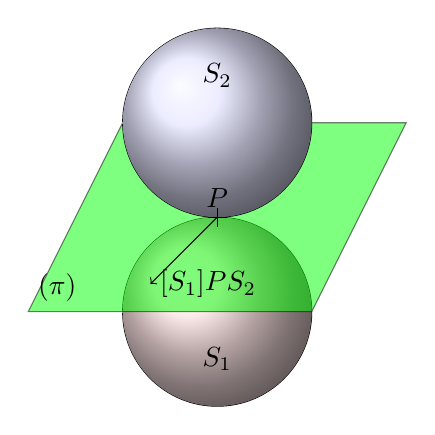
\begin{tikzpicture}[scale=1.2]
		    \draw (0,0) circle (1cm);
		    \shade[ball color=red!10!white] (0,0) circle (1);
		    \draw[fill=green,opacity=0.5] (-1,2) --++ (-1,-2) node[opacity=1,anchor=south west]{$(\pi)$} --++ (3,0) --++ (+1,+2) -- cycle;
		    \draw (0,2) circle (1cm);
		    \shade[ball color=blue!10!white] (0,2) circle (1);
		    \coordinate (P) at (0,1);
		    \draw (P)--++(0.1,0);
		    \draw (P)--++(-0.1,0);
		    \draw (P)--++(0,0.1);
		    \draw (P)--++(0,-0.1);
		    \node[anchor=south] at (P){$P$};		
			\node at (0,-0.5){$S_1$};    
			\node at (0,2.5){$S_2$};
			\draw[->] (P)-- ++ (-135:1) node[anchor=west]{$\V[S_1]{P}{S_2}$};  
		\end{tikzpicture}
	\end{minipage}
	\begin{minipage}[b]{0.5\textwidth}
		\begin{definition}
	Soient deux solides $S_1$ et $S_2$, en contact mutuel en $P$. On appelle vecteur de glissement de $S_2$ par rapport à $S_1$ le vecteur vitesse $\V[S_1]{P}{S_2}$.
		\end{definition}
	
	\begin{theorem}
		Soit $(\pi)$ le plan tangent à $S_1$ et à $S_2$ en $P$. $\V[S_1]{P}{S_2}$ est alors compris dans le plan $(\pi)$. C'est la condition dite de non-pénétration.
	\end{theorem}	
	\end{minipage}
	

	\subsection{Roulement sans glissement}
	\begin{definition}
		On dit que $S_2$ roule sans glisser sur $S_1$ si et seulement si :
		\hidden{
		\begin{equation}
			\V[S_1]{P}{S_2}=\vect{0}
		\end{equation}
		}
	\end{definition}
	
\section{Rotations de roulement et de pivotement}
	\begin{wrapfigure}{r}{0.4\textwidth}
		\begin{tikzpicture}[scale=1.2]
		    \draw (0,0) circle (1cm);
		    \shade[ball color=red!10!white] (0,0) circle (1);
		    \draw[fill=green,opacity=0.5] (-1,2) --++ (-1,-2) node[opacity=1,anchor=south west]{$(\pi)$} --++ (3,0) --++ (+1,+2) -- cycle;
		    \draw (0,2) circle (1cm);
		    \shade[ball color=blue!10!white] (0,2) circle (1);
		    \coordinate (P) at (0,1);
		    \draw (P)--++(0.1,0);
		    \draw (P)--++(-0.1,0);
		    \draw (P)--++(0,0.1);
		    \draw (P)--++(0,-0.1);
		    \node[anchor=north west] at (P){$P$};		
			\node at (0.5,-0.5){$S_1$};    
			\node at (0.5,1.5){$S_2$};
			\draw[-latex,very thin] (P)-- ++ (0,2.3) node[anchor=west]{$\vect{n}$}; 
			\coordinate (Om) at (-0.5,2);
			\coordinate (Pn) at (0,2.2);
			\coordinate (Pp) at (-0.5,0.6);
			\draw[blue,thick,-latex] (P) --(Om) node[anchor=east]{$\Om[S_1]{S_2}$};
			\draw[red,very thick,-latex] (P) --(Pn) node[anchor=south]{$\vect{\Omega}_{{n}}(\nicefrac{S_2}{S_1})$};
			\draw[red,very thick,-latex] (P) --(Pp) node[anchor=north]{$\vect{\Omega}_{\mathrm{t}}(\nicefrac{S_2}{S_1})$};
			\draw[very thin, dashed,red] (Pn) -- (Om) -- (Pp);
		\end{tikzpicture}
	\end{wrapfigure}
On note $\vect{n}$ le vecteur normal au plan $(\pi)$. On peut décomposer le vecteur vitesse de rotation de $S_2$ par rapport à $S_1$ selon :
\begin{description}
	\item[une rotation de pivotement] portée par $\vect{n}$ et notée $\vect{\Omega}_{{n}}(\nicefrac{S_2}{S_1})$.
	\item[une rotation de roulement] comprise dans le plan $(\pi)$ et notée $\vect{\Omega}_{\mathrm{t}}(\nicefrac{S_2}{S_1})$.
\end{description}
On a donc :
\begin{equation}
	\Om[S_1]{S_2}=\vect{\Omega}_{{n}}(\nicefrac{S_2}{S_1})+\vect{\Omega}_{\mathrm{t}}(\nicefrac{S_2}{S_1})
\end{equation}


\newpage
\section{Composition des accélérations}
\begin{theorem}
	\hidden{
	Soit un solide $S$ en mouvement par rapport à un repère $\Rc_1$, lui-même en mouvement par rapport à un repère $\Rc_0$. On note $P$ un point de $S$. On a alors :
	\begin{equation}
		\G[\Rc_0]{P}{S}=\G[\Rc_1]{P}{S}+\G[\Rc_0]{P}{\Rc_1}+2\Om[\Rc_0]{\Rc_1}\wedge\V[\Rc_1]{P}{S}
		\label{eq:compo-acceleration-th}
	\end{equation}
	}
\end{theorem}
Les composantes de cette équation sont :
\begin{description}
	\item[L'accélération absolue] $\G[\Rc_0]{P}{S}$
	\item[L'accélération relative] $\G[\Rc_1]{P}{S}$
	\item[L'accélération d'entraînement] $\G[\Rc_0]{P}{\Rc_1}$
	\item[L'accélération de Coriolis] $2\Om[\Rc_0]{\Rc_1}\wedge\V[\Rc_1]{P}{S}$
\end{description}

\begin{proof}
	En dérivant l'expression~\eqref{eq:compos-vitesse} on trouve :
	\begin{equation}
		\label{eq:fat-derivation}
		\begin{split}
		\diff[\Rc_0]{\V[\Rc_0]{P}{S}}=\diff[\Rc_0]{\V[\Rc_0]{O_1}{\Rc_1}}+\diff[\Rc_0]{\Om[\Rc_0]{\Rc_1}}\wedge\vect{O_1P}\\
		+\Om[\Rc_0]{\Rc_1}\wedge\diff[\Rc_0]{\vect{O_1P}}+\diff[\Rc_0]{\V[\Rc_1]{P}{S}}
		\end{split}
	\end{equation}
	Par définition de l'accélération, on sait que :
	\begin{subequations}
		\label{eq:calcul-gamma}
		\begin{align}
			\diff[\Rc_0]{\V[\Rc_0]{P}{S}}&=\G[\Rc_0]{P}{S}\\
			\diff[\Rc_0]{\V[\Rc_0]{O_1}{S}}&=\G[\Rc_0]{O_1}{S}
		\end{align}
	\end{subequations}
	Par ailleurs :
	\begin{align}
		\Om[\Rc_0]{\Rc_1}\wedge\diff[\Rc_0]{\vect{O_1P}}&=\Om[\Rc_0]{\Rc_1}\wedge\left(\diff[\Rc_1]{\vect{O_1P}}+\Om[\Rc_0]{\Rc_1}\wedge\vect{O_1P}\right)\\
														&=\Om[\Rc_0]{\Rc_1}\wedge\V[\Rc_1]{P}{S}+\Om[\Rc_0]{\Rc_1}\wedge\left(\Om[\Rc_0]{\Rc_1}\wedge\vect{O_1P}\right)
														\label{eq:omega-vect-diff}
	\end{align}
	et :
	\begin{align}
		\diff[\Rc_0]{\V[\Rc_1]{P}{S}}	&=\diff[\Rc_1]{\V[\Rc_1]{P}{S}}+\Om[\Rc_0]{\Rc_1}\wedge\V[\Rc_1]{P}{S}\\
										&=\G[\Rc_1]{P}{S}+\Om[\Rc_0]{\Rc_1}\wedge\V[\Rc_1]{P}{S}
										\label{eq:deriv-inconnue}
	\end{align}			
	En remplaçant les termes de l'équation~\eqref{eq:fat-derivation} par ceux déterminés en \eqref{eq:calcul-gamma}, \eqref{eq:omega-vect-diff} et \eqref{eq:deriv-inconnue}, on trouve :
	\begin{equation}
		\label{eq:fat-derivation2}
		\begin{split}
			\G[\Rc_0]{P}{S}=
			\G[\Rc_0]{O_1}{S}
			+\diff[\Rc_0]{\Om[\Rc_0]{\Rc_1}}\wedge\vect{O_1P}
			+\Om[\Rc_0]{\Rc_1}\wedge\left(\Om[\Rc_0]{\Rc_1}\wedge\vect{O_1P}\right)\\
			+\G[\Rc_1]{P}{S}
			+2\Om[\Rc_0]{\Rc_1}\wedge\V[\Rc_1]{P}{S}
		\end{split}
	\end{equation}
	Or on a vu en~\eqref{eq:composition-accelerations} que :
		\begin{equation}
			\G[\Rc_0]{P}{S}=\G{O_1}{S}+\diff[\Rc_0]{\Om{S}}\wedge\vect{O_1P}+\Om[\Rc_0]{S}\wedge\left(\Om[\Rc_0]{S}\wedge\vect{O_1P}\right)
		\end{equation}
	On peut donc simplifier l'équation~\eqref{eq:fat-derivation2} pour aboutir à l'équation~\eqref{eq:compo-acceleration-th}.
\end{proof}
